% Copyright (C) 2019 Cui Jialiang ( SESS, PKU ). All rights reserved.

\chapter{基于CNN和RNN的像素级别跟踪算法}
本章是本文的重点,将详细介绍本研究的理论创新.
\par
本研究所作的重点工作实际上是运用了深度学习技术,结合加密-解码结构的图像分割算法,加入RNN等结构实现了像素级别目标跟踪.具体算法结构,实现细节,训练等将在本章重点介绍.本章后文中将称本研究中提出的基于CNN和RNN的像素级别跟踪算法为本算法.

\section{算法简介}
本算法将首先基于用于实现静态图像分割的U-Net\supercite{ronneberger2015u}的多级降级-升级卷机神经网络结构.和处理静态图片的图像分割算法不同,我们将在这个多级网络结构中加入Conv-LSTM结构.
\par
与纽约大学2017年实现的Conv-LSTM结构的跟踪算法不同的是,本文所采用的多级神经网络将把Conv-LSTM加入各个卷机层级;而与U-Net,SegNet等多级分割算法不同的是,本文将在整个结构中多处穿插LSTM以得到一个时间连续的结果.
\par
同大多数跟踪算法类似,本算法的输入是一张张图片组成的视频序列,输出是像素级的跟踪结果.处理过程中需要始终存储并更新跟踪状态.
\par
本算法的结构如图\ref{fig:space_process},\ref{fig:CNN_FCLSTM},\ref{fig:time_process}所示.

\par
\begin{sidewaysfigure}[htbp!]
    \centering
    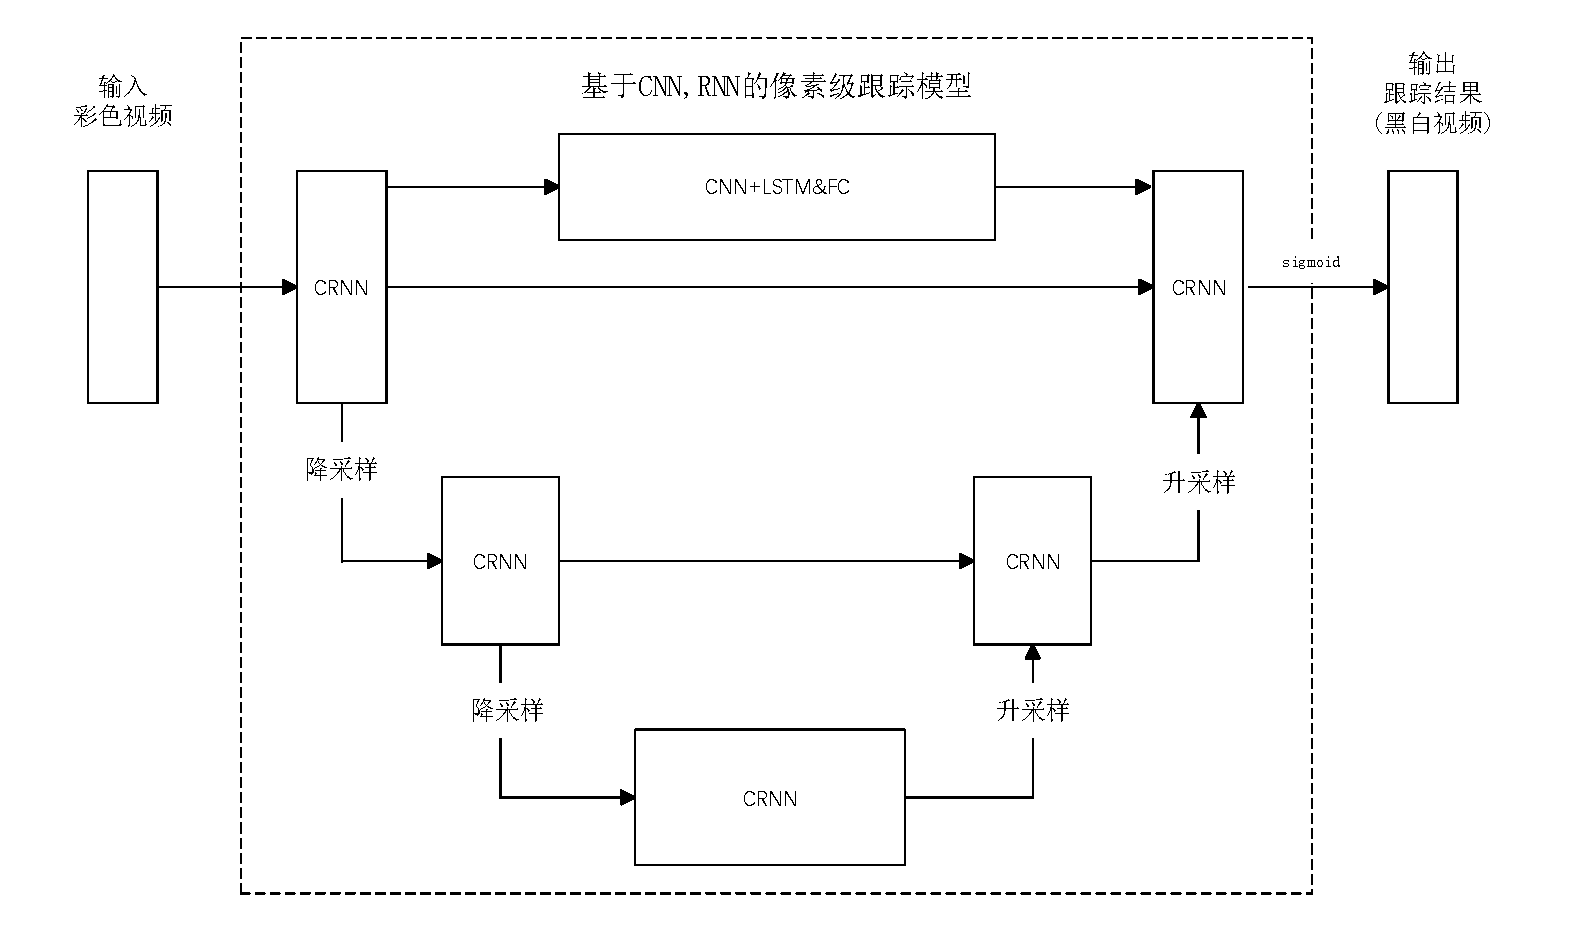
\includegraphics[width = 1.\textwidth]{chap/img/space_process.pdf}
    \caption{本算法在空间维度对单张图片的处理(这里略去了处理时间维度的RNN)}
    \label{fig:space_process}
\end{sidewaysfigure}
\par
\begin{figure}[htbp!]
    \centering
    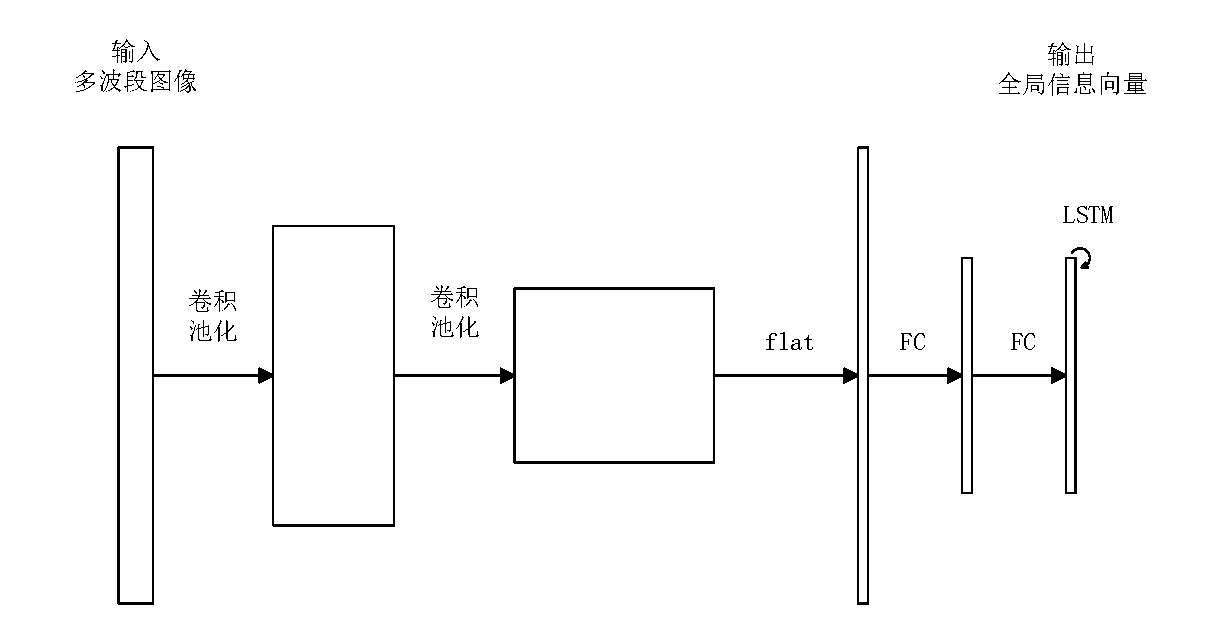
\includegraphics[width = 1.\textwidth]{chap/img/CNN_FCLSTM.pdf}
    \caption{处理宏观信息的CNN+LSTM\&FC结构}
    \label{fig:CNN_FCLSTM}
\end{figure}
\par
\begin{sidewaysfigure}[htbp!]
    \centering
    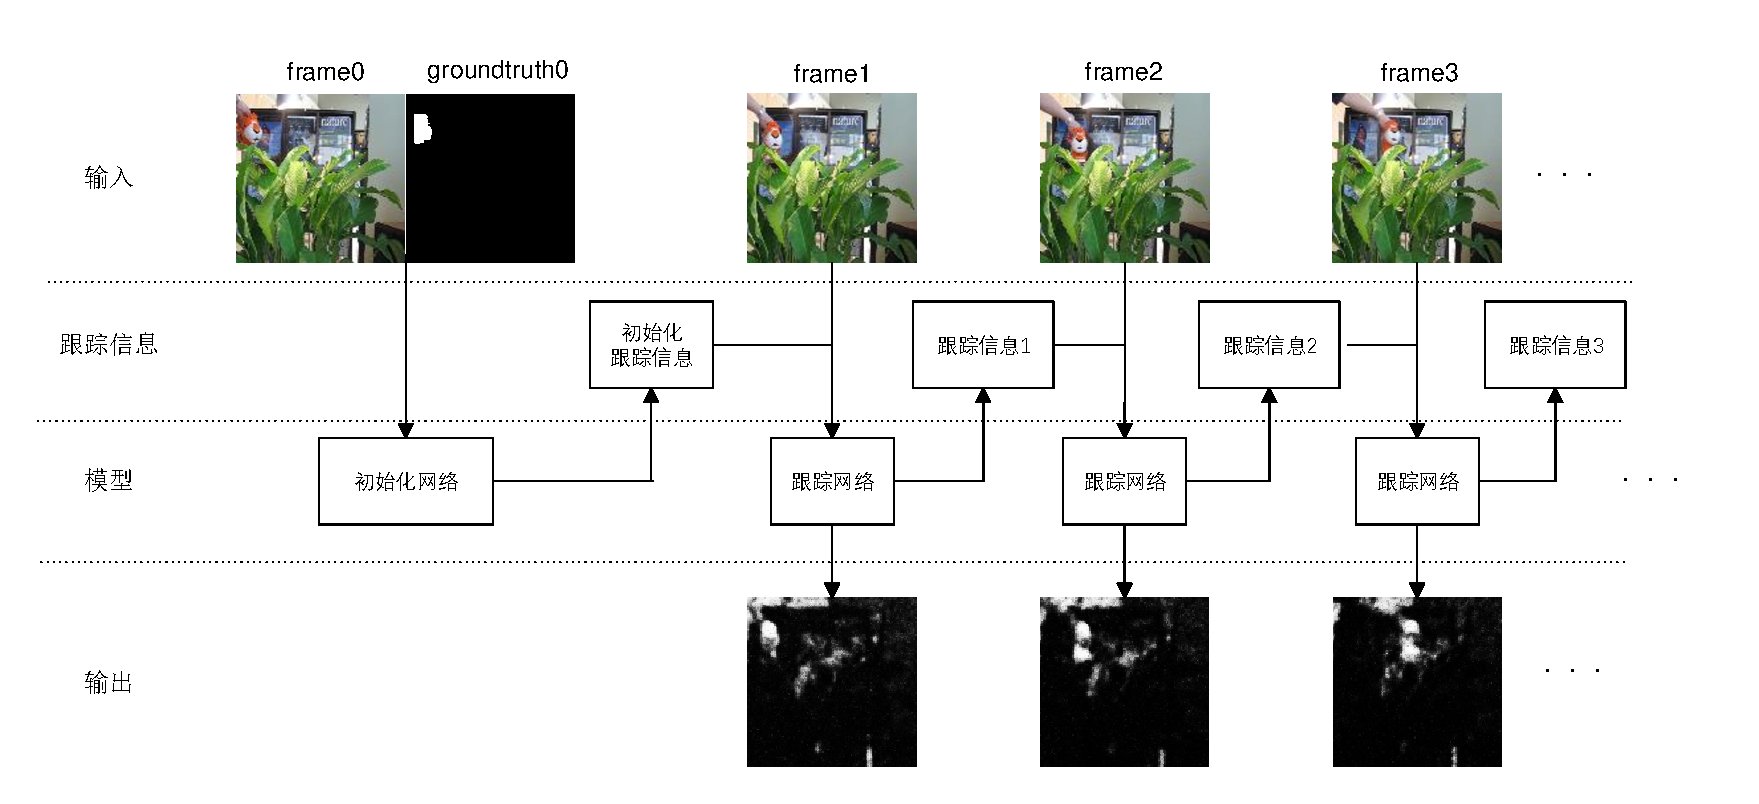
\includegraphics[width = 1.\textwidth]{chap/img/time_process.pdf}
    \caption{本算法在时间维度的大致处理思路}
    \label{fig:time_process}
\end{sidewaysfigure}
\par

\subsection{算法的输入} \label{section:input_of_our_algorithm}
\par
在输入阶段,RGB传感器得到的图像由三张原图大小的灰度图像组成.不同于SIFT\supercite{lowe1999object},SURF\supercite{bay2006surf}等一些视觉图像处理算法,得益于深度学习方法在张量理解的优势,本算法将直接接受多波段的彩色图片为输入,这样能获得更大的输入空间.
\par
事实上,由于该输入需要被送入深度神经网络,为了更好的得到归一化的训练结果,本算法在输入阶段需要对输入数据进行归一化至$[0,1]$.对于三个波段都在$[0,255]$取值范围内的一个简单的归一化方法是:
\par
\begin{equation}\label{equ:input_norm}  input_{normlized} = \frac{input_{origin}}{255}  \end{equation}
\par
由于本算法的CNN处理过程中需要将2D图像结果展开(flat)后输入FC层,本算法只能接受固定输入大小的输入.本文后文的实验中将所有输入数据采样调整大小(Resize)至$500*500$大小的图片后进行处理.事实上如果不加入Conv+LSTM\&FC结构,本算法可以接受任意大小的输入.
\par

\subsection{算法的输出}
本算法的输出是像素级的跟踪结果.像素级的跟踪结果将用一幅图像表示,高亮的像素代表目标,黑暗的像素代表背景.
\par
实际上本算法的输出由于经过Softmax\footnote{实际是Sigmoid}(软间隔最大化)处理,得到的所有像素的结果都将位于$(0,1)$间,某个像素的结果意味着该像素是目标的概率.由于通常得到的结果置信度不高,该结果很多情况下可以直接加以应用.如果希望得到严格区分的二分类结果,可以选择一个阈值(如$0.5$)将结果二值化.

\subsection{处理时效性}
本算法实际上是一个可以实时执行的跟踪算法.对于一个待提取跟踪目标的视频,本算法产生结果并不需要读入整个视频,只需输入当前与之前时刻的帧即可.即在跟踪过程中,每读入一张图片即进行一次处理.这使得在拥有一定量的计算资源时,本算法可以进行实时处理,即接收的图像结果的同时给出跟踪结果.

\subsection{时间复杂度}
对于$n$帧的视频,本算法的时间复杂度是$O(n)$,即增加视频长度只会线性增加算法处理所需的时间.
\par
对于不同大小的输入视频,由于在\ref{section:input_of_our_algorithm}中提到的对输入进行大小的调整,本算法对所有大小的视频处理速度相同.如果希望变化处理大小以得到更精细的结果,对于大小为$n*m$的调整后的输入,本算法的时间复杂度将是$O(n*m)$.


\section{本算法在时间维度的处理}
\par
本算法在时间尺度主要依靠RNN技术处理.有关RNN的基础概念已在\ref{section:rnn}中介绍过.
\par
本研究的算法将主要采用LSTM算法解决问题.具体的,LSTM单元将被加入到各个层级当中.LSTM在各种跟踪算法中有广泛应用,但大多数算法仅仅将其作为对最后结果的处理手段.本研究的算法将把LSTM作为所有的中间状态记录单元.

\subsection{跟踪状态}
\par
\begin{sidewaysfigure}[htbp!]
    \centering
    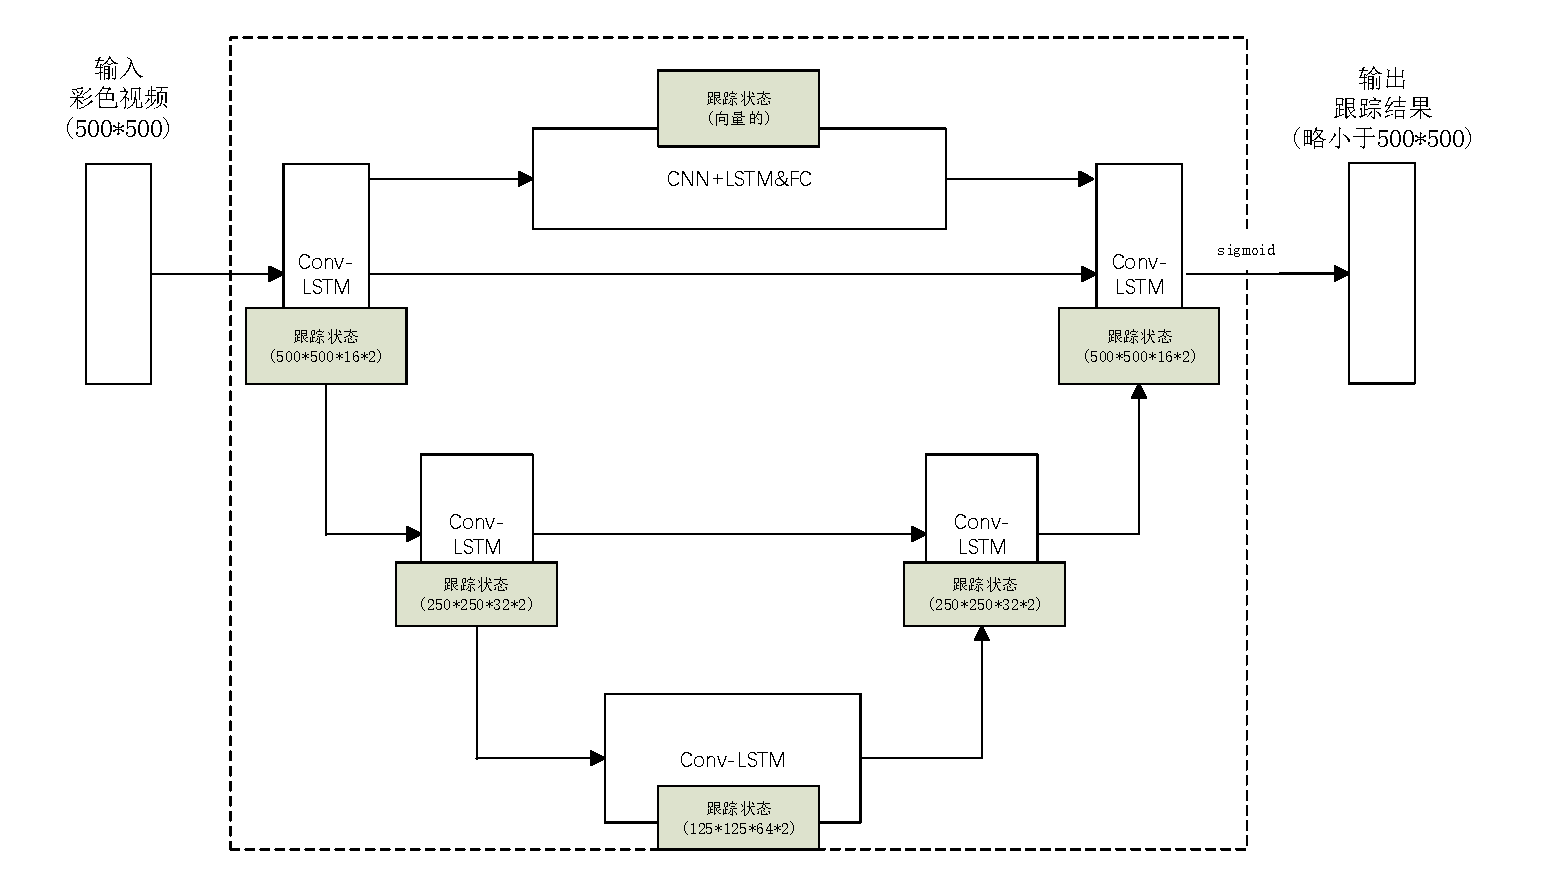
\includegraphics[width = 1.\textwidth]{chap/img/tracking_state.pdf}
    \caption{以500*500大小输入为例,所有跟踪状态大致形状}
    \label{fig:tracking_state}
\end{sidewaysfigure}
\par
前文\ref{section:tracking_state}中介绍过视频跟踪算法中\textbf{跟踪状态}的概念.本算法直接使用RNN状态量记录和使用跟踪状态.当使用LSTM时,RNN的$h$和$c$状态量将同时作为跟踪状态使用.
\par
本算法的需要记录的所有跟踪状态大致如图\ref{fig:tracking_state}所示.前文中介绍过,跟踪状态的物理意义是之前的运动状态.由于加密-解码结构的多尺度效果(\ref{section:multiscale}中有介绍),这些跟踪状态也对应多尺度的物理含义.Conv+LSTM\&FC中的跟踪状态对应最全局的信息;自上而下,低级的跟踪状态代表细节,微观的信息,高级的跟踪状态代表宏观信息.
\par
这个多级别的跟踪状态的设计是本文的核心思想所在,本算法其他结构也是围绕着维护这些跟踪状态设计的.

\subsection{跟踪状态初始化}
\textbf{跟踪状态初始化}指在跟踪初始如何获取一开始的跟踪状态.本算法使用一个\textbf{初始化网络}进行跟踪状态初始化,初始化网络的使用如图\ref{fig:time_process}中所示.
\par
初始化网络接受的输入是第一帧图像和第一帧图像的标记,输出初始化生成的所有跟踪状态,本算法的所有计算过程也从此开始.
\par
初始化网络使用和后续处理类似的结构,但参数不同.训练时将同时训练两个网络.由于该网络功能上和跟踪网络差异较大,很难实现共享参数.
\par
需要注意的是,如果后续的Block-RNN结构使用LSTM作为RNN单元,则初始化网络输出的结果需要适配LSTM的状态量大小,即普通RNN的状态量的两倍大小.

\section{本算法在空间维度的处理}
本节与下一节将详细介绍本算法在空间,时间维度处理的设计理念.
\par
本算法处理空间维度的思路来源于U-Net\supercite{ronneberger2015u}.事实上近年来几乎所有的像素级别处理都参考了该结构.
\par
类似与U-Net的结构,本文的卷机网络部分也将有多个降级和升级结构;每个降级结构包括几个卷积层,使用池化结构进行降级;每个升级部分采用升卷积进行升级处理.在降级过程中,图片数据的尺寸大小会衰减,同时等比例增加其波段范围.对于3层的结构,最小级的波段将有128个.

\subsection{多尺度处理思想} \label{section:multiscale}
这个多级结构的设计理念是为了处理多尺度问题.
\par
浅层的级别能很好的处理细节问题,但对宏观的把控会较弱,具体表现为可能会出现噪声点;深层的结构对宏观把控好,但对边界处理较弱.升级结构能将浅层处理得到的边界信息与深层处理得到的宏观信息相结合,得到一个更好的结果.

\subsection{块状卷积循环神经网络} \label{section:crnn}
前文\ref{section:cnn}中介绍过CNN(卷积神经网络)的结构.几乎所有处理图像的深度神经网络都有CNN结构.本文使用其变种,结合RNN的块状卷积循环神经网络来处理空间维度问题.